\documentclass[../main.tex]{subfiles}
\begin{document}

\section{General Information}
Below is some general information about components and helpful keywords. 

\subsection{Dice}
Dice will be referenced throughout the game starting with the quantity and concluding with the type. For instance, six- sided dice will be referenced a both D6 and 2D6, where the D6 indicates the type of dice to use and the 2 indicates how many of that dice to use. 

\subsubsection{Combat Dice}
\begin{figure}[h]
    \centering
    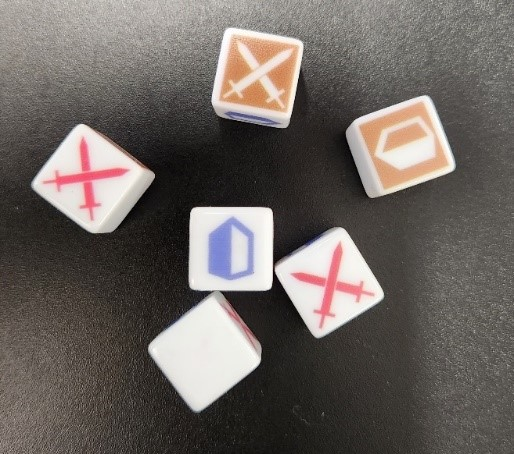
\includegraphics[width=0.75\linewidth]{chapters//generalInformation/TimeStrikeCombatDice.jpg}
\end{figure}

These 6- sided dice are referred to as Combat Dice or D6 and are primarily used to resolve combat. These dice have three sides showing an Attack Icon (crossed swords), two sides showing a Defense icon (shield), and one blank side. One Attack side and one Defense side is also marked as Lucky, with a golden background. Certain characters will make use of Lucky Attack or Lucky Defense rolls within their skillsets. 

\subsubsection{D20}
\begin{figure}[h]
    \centering
    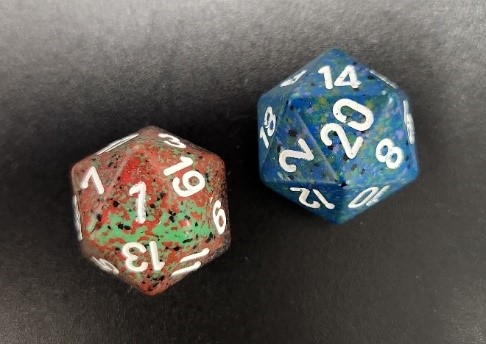
\includegraphics[width=0.90\linewidth]{chapters//generalInformation/TimeStrikeD20Dice.jpg}
\end{figure}
These 20-sided dice are referred to as D20s and are used in all other aspects of the game. When using a D20, the default mechanic is to roll a 10 or higher to succeed in any action unless otherwise specified. If players are rolling D20s against each other, all ties are re-rolled unless otherwise specified. 

\subsubsection{Markers}
Marker cubes will be used to track changes to Characters throughout the game. Each Character card has cut slots in columns: Heath Bar, Buff, Curse, and Awakened stats. The marker cubes fit into these slots. 
On a new Character, slots begin filled to represent stats that are not active and will be removed, revealing the stat beneath, indicating that it is activated. If a box is gray, than that stat can nver be active, and it should remain empty. 
\begin{figure}[h]
    \centering
    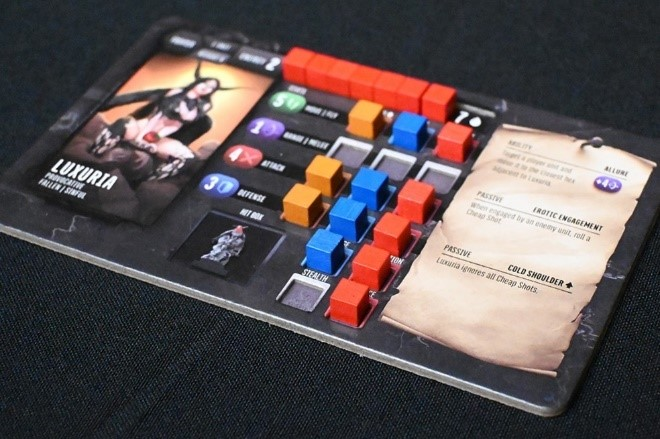
\includegraphics[width=1\linewidth]{chapters//generalInformation/TimeStrikeCharacterCardSlotsMarkers.jpg}
    \caption{Character Card with curses, buffs, and damage taken. Gray cut slots are left empty.}
\end{figure}
\subsection{Walls}
Walls can be built throughout the game using materials. They allow the player to obstruct line of sight, block passageways, and negate incoming attacks. 

\subsection{Sentience Mobs}
Each Sentience will have miniatures included which are tied to the mechanics of that specific Sentience. These will be referred to as the Sentience mobs. 

\subsection{Hexes}
Hexes are either land hexes or tile hexes. Hexes (and anything occupying them) are considered adjacent if they are next to each other, regardless of any height difference. 

There are three types of land hexes included in this set: basic sand tiles, obsidian/red rock resources hexes, and stone/concrete road hexes. 

Water is the only type of tile hex included in this set. Tile hexes are considered to be one hex lower in elevation than land hexes. 

\clearpage
\end{document}